\chapter{Background}
\section{Merkle tree}
Ralph Merkle invented the merkle trees in 1979. We present here the binary merkle tree used in bitcoin and a derivation of the patricia merkle tree used in ethereum.
\subsection{Binary merkle tree}
\begin{figure}[H]
    \centering
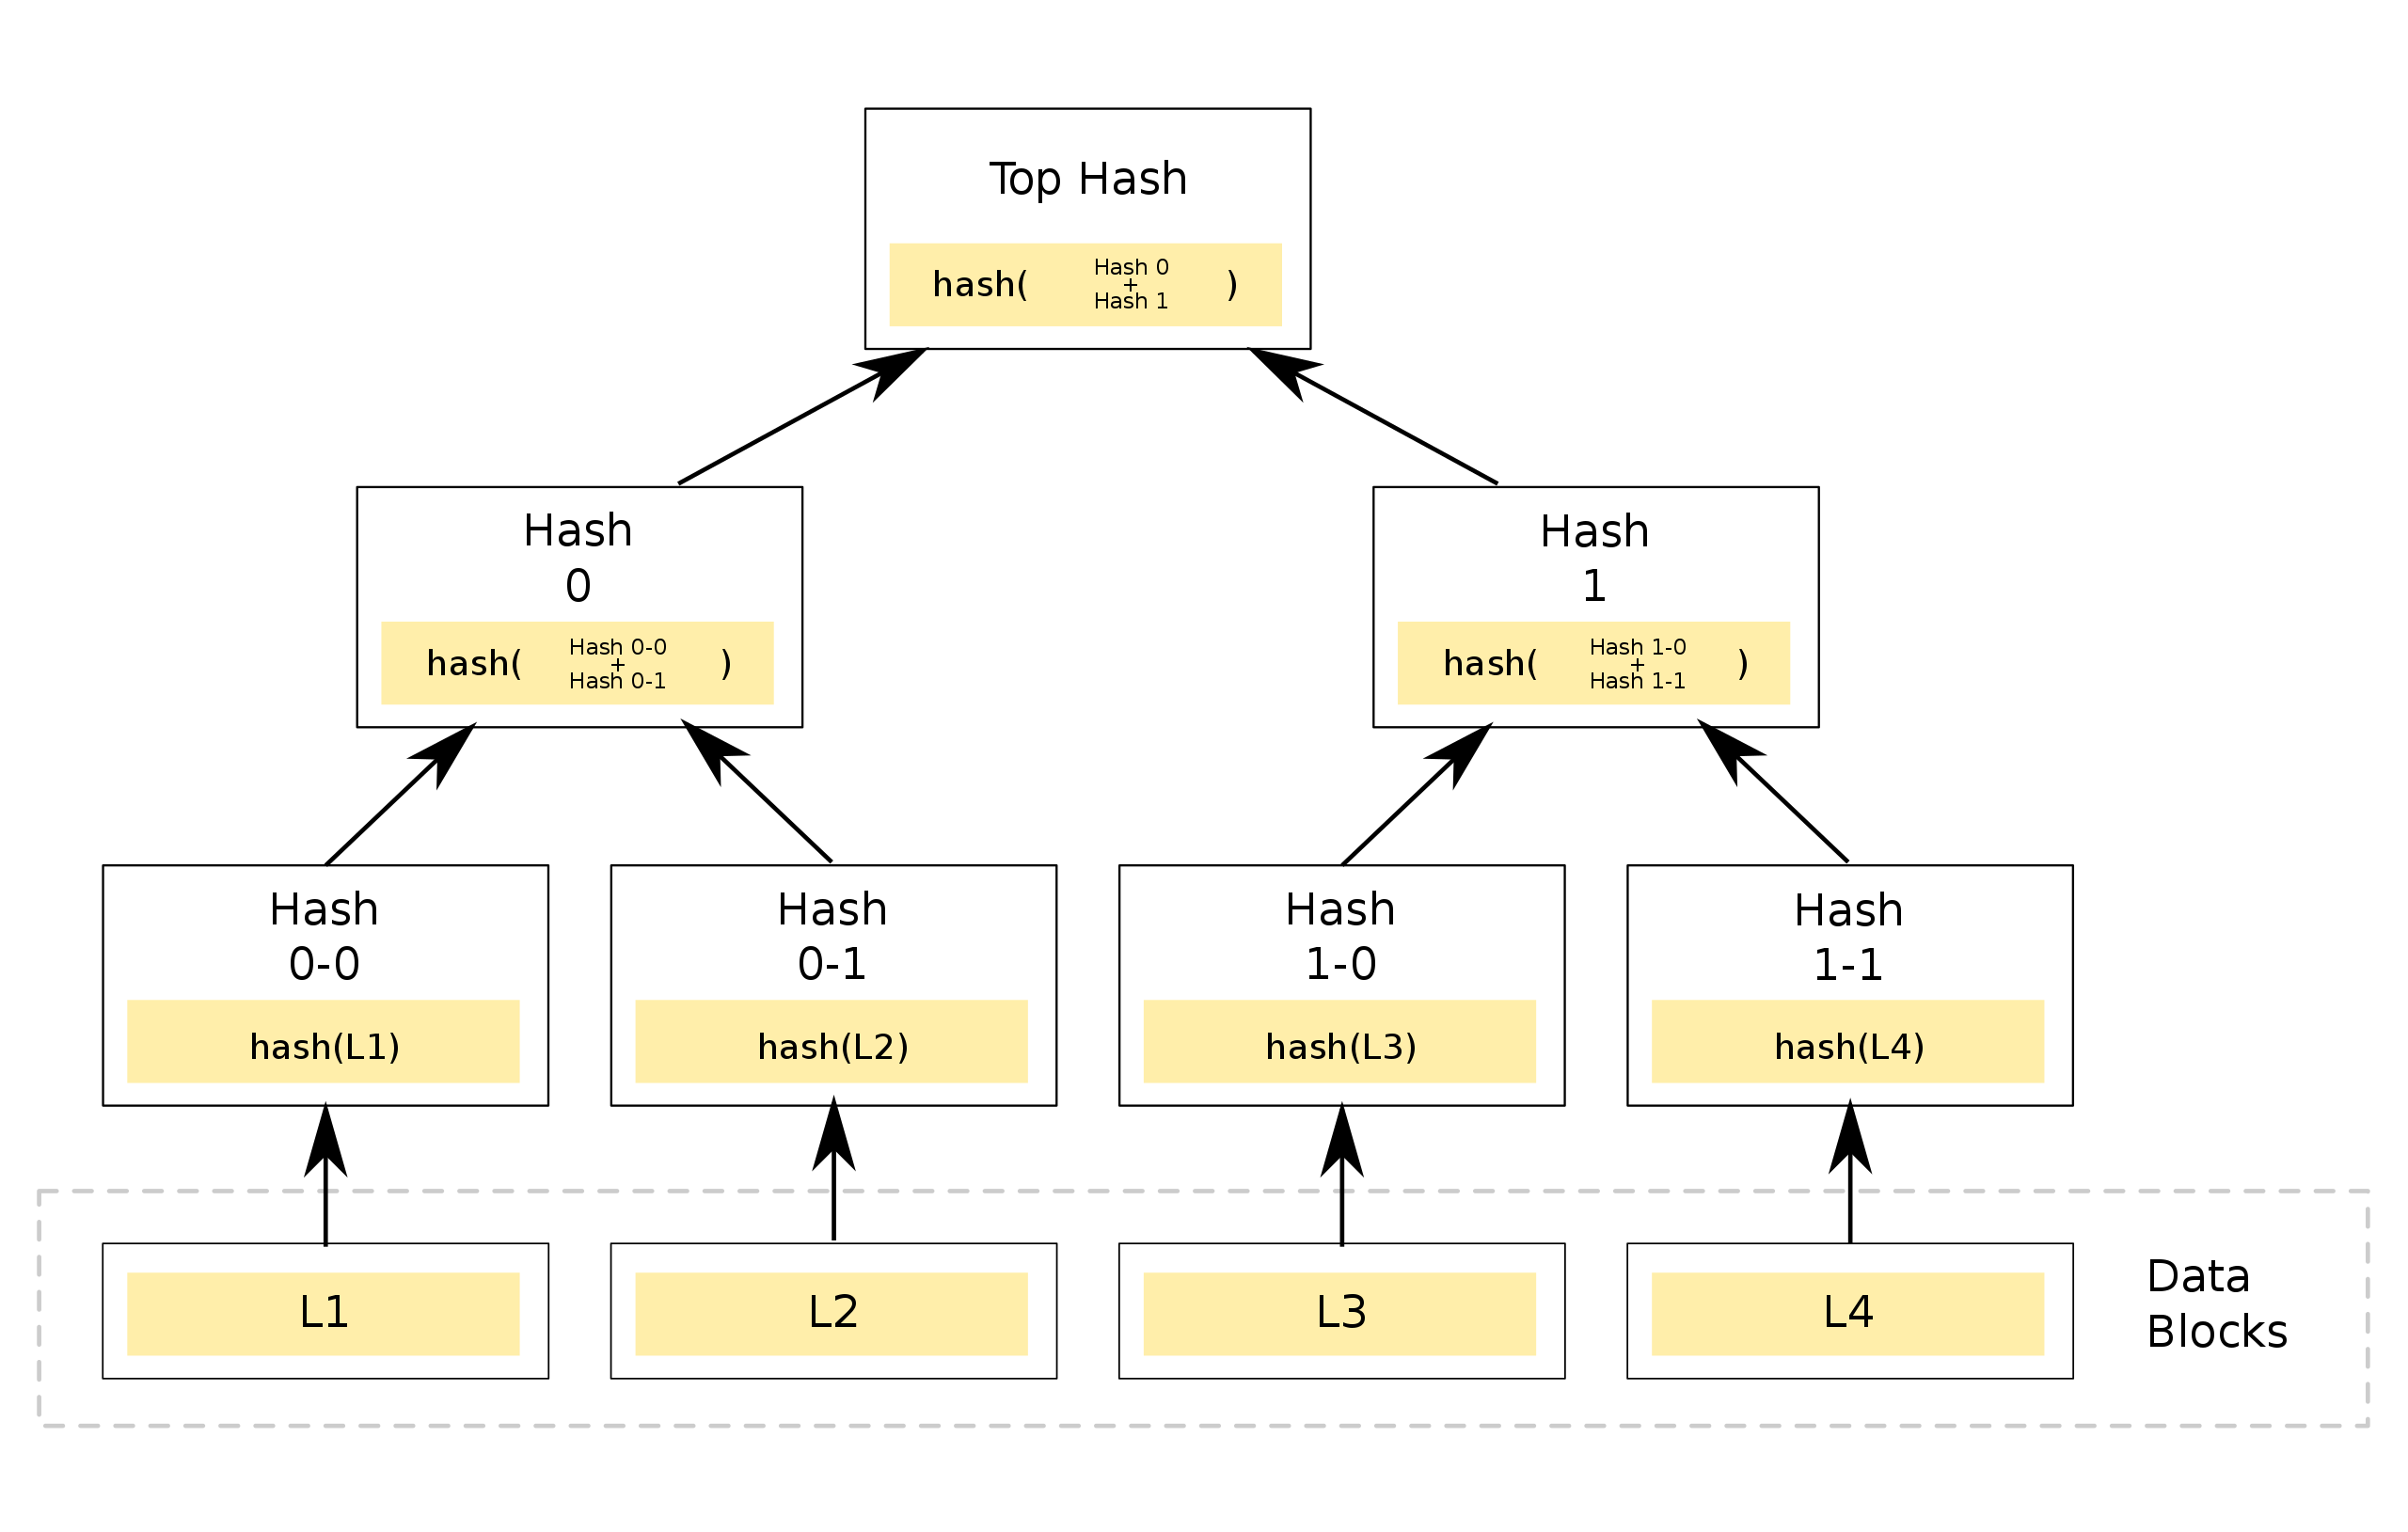
\includegraphics[width=0.7\linewidth]{background/merkle.png}
    \caption{Binary merkle tree}
    \label{fig:merkle}
\end{figure}
The binary merkle tree consists of hashing the transaction two by two: 
\begin{enumerate}
    \item List all the data you want to save in an ordered list: it can be n users for example or any kind of data. In blockchain, these data are the transactions. Here say we have 4 transactions L1, L2, L3, L4.
    \item Hash these data one by one to obtain n hashes. Here we obtain 4 transactions hashes \\($Hash_{0-0},Hash_{0-1},Hash_{1-0},Hash_{1-1})$
    \item Hash the hashes two by two starting from the left. If there is only one node on the right of the tree, we duplicate it two obtain the parent. Here we obtain $Hash_0, Hash_1$.
    \item Repeat the last step until we obtain only one node left: the root.
\end{enumerate}
The root is a fingerprint of all the data, in our case the four transactions. 
It means that if you change anything in the original data, the timestamp of the first transaction for example, it'll change completely the root hash of the merkle tree, thanks to the non locality property of the hash function used (Alice and Aline have very different hashes even if they have only one different letter)

\subsection{Proof of inclusion} \label{merkle:inclusion}
Merkle trees allow to summarize the data into one fixed length fingerprint, the root hash. 
But why should we use this data structure instead of just hashing all the hashes for example?

This data structure allows proof of inclusion. In the case of bitcoin for example, data is the transactions, and this structure allows other users to answer this question: \\
\textbf{Is this transaction really included in that block?}

So let's consider the merkle tree below:

\begin{figure}[H]
  \centering
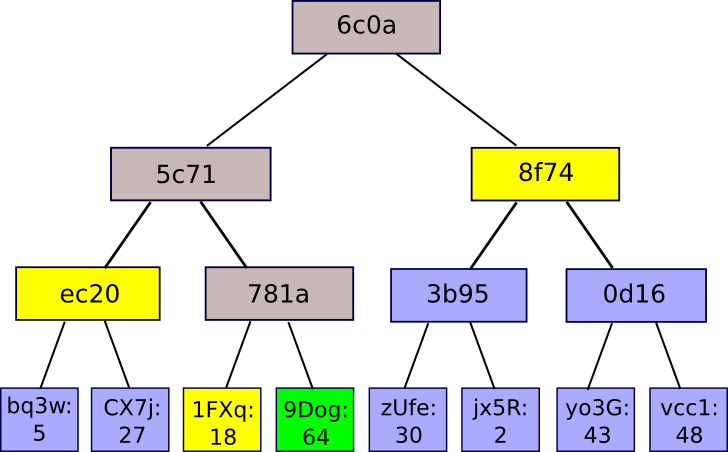
\includegraphics[width=0.5\linewidth]{background/merkle_proofs_2.png}
\caption{Proof of inclusion in merkle tree}
\end{figure}

We have 8 transaction hashes that we want to place in the merkle tree in this example. Let's say we are interested in the transaction in green (9Dog:64) because it's directed to our account. We want a proof that this transaction has really happened, and have been included in that block with merkle root 6c0a. 

The proof is a merkle block with the yellow hashes. The verifier of this proof can then follow these steps:
\begin{enumerate}
    \item With green transaction and the yellow one 1FXQ:18 you can concatenate and hash it to get the parent hash 781a.
    \item With this last hash 781a and the yellow one ec20 you can concatenate and hash them to get the parent hash 5c71.
    \item And with this last hash concatened with the last yellow one 7f74 and hashed, we get the merkle root
    \item We compare the calculated merkle root from the proof and the real one from the block. If they match, the proof is accepted.
    In bitcoin, it means that the transaction is included in this block. If they don't , we cannot prove the inclusion with that proof. 
\end{enumerate} 

\textbf{
What is the advantage of using this data structure?}

The verifier only needs the merkle root of the block to accept the proof of inclusion. But as this is a binary tree, the number of hashes at each level is divided by two, so this proof only consists of $\log_2(n)$ hashes, with n the number of transactions. 
It means that if we have 8 transactions, as in this example we  need one hash per level so $\log_2(8)=3$ hashes to proof the inclusion of the transaction in the block.

\colorbox{lime}{
\textbf{
If $n=100$ we need $\log_2(100)\sim 7$ hashes, if $n=1000$ we need $\log_2(1000)\sim 10$ hashes.
}
}


\section{Blockchain basics}

The blockchain can be viewed as a replicated state machine. It means that  each time $t$ is associated with a global state which goes to the next state at $t+1$ with the state transition function. 

Here the state is for example account balances for bitcoin, the state transition function represented by the transactions, instructions to be executed to go to the next state.
In blockchain, the transactions for each state transition are placed in a new block, adding to the chain of blocks.
\begin{figure}[H]
\centering
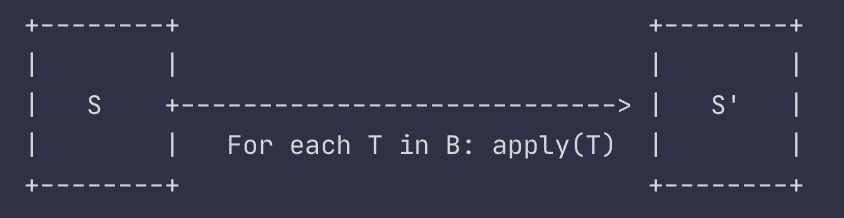
\includegraphics[width=0.6\linewidth]{background/state_transition.png}
    \caption{The state S transitioning to state S' by executing all transactions T from the block B}
    \label{fig:state_transition}
\end{figure}
Lastly, it is replicated across all the full nodes to ensure global consistency of the distributed ledger, meaning that the nodes on the network should agree on the blockchain state thanks to the consensus algorithm.

\subsection{The block}
So what is stored exactly in a block? 

Let's say for the moment that the bitcoin block consists of:
\begin{itemize}
    \item the hash of the previous block. You take the whole previous block and pass it to the hash function.
    \item the nonce resulting from the cryptographic puzzle. We'll talk about it later. 
    \item the list of transactions included in the block.
\end{itemize}
\begin{figure}[H]
    \centering
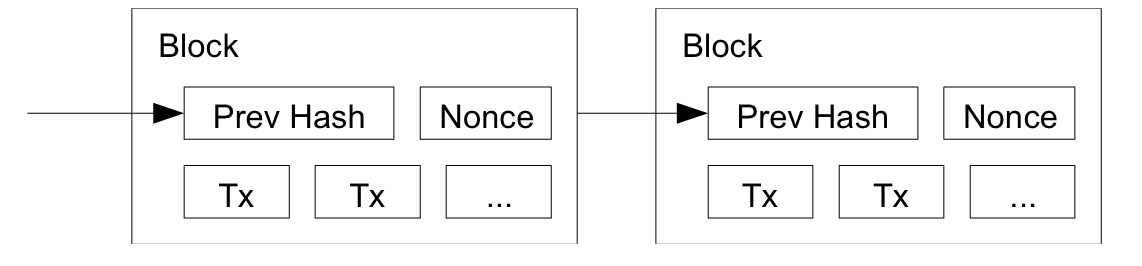
\includegraphics[width=0.6\linewidth]{background/block.png}
    \caption{A bitcoin block: the hash of the previous block, the nonce, and the list of transactions}
    \label{fig:block}
\end{figure}

This requires every node in the network to keep the list of transactions since 2009.

\subsection{Merkle tree of transactions}
In fact, the block is composed of the block header and the list of transactions. The block header contains this time the root hash of the transactions merkle tree.
The root hash is a summary of all the transactions happening during that period represented a merkle tree. For bitcoin, binary merkle tree are used for transactions, whereas in Ethereum, merkle Patricia trees are used to store transactions, state, receipts. 
\begin{figure}[H]
    \centering
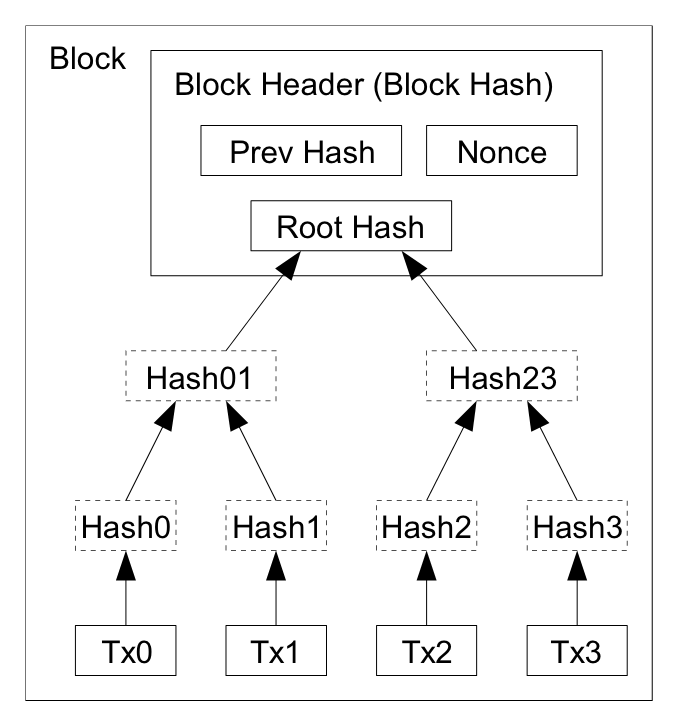
\includegraphics[width=0.4\linewidth]{background/blockmerkle.png}
    \caption{A Bitcoin\cite{Nakamoto..09} block}
    \label{fig:blockmerkle}
\end{figure}

\subsection{Single payment verification}
This allows two actors to emerge: \\
\textbf{The full node} stores all the full blocks, with the transactions. With this transactions, it can provide the proof of inclusion: the hashes required to prove a transaction is in a particular block. \\
\textbf{The light node } asks for the blocks headers to the full nodes of the network. Once he got the block headers, he can ask the full nodes of the network to provide a proof for the transactions is interested into. With the procedure described in \ref{merkle:inclusion}, the light node can verify that the transaction has indeed happened in the blockchain.

The light node is only storing the block headers, so even a phone can handle the amount of storage needed. This allows for example to verify with your wallet that a transaction has been executed  on your laptop without downloading the $\sim 500$GB of the blockchain.


